\documentclass[tikz]{standalone}
\usepackage{fontspec}
\renewcommand*{\familydefault}{\sfdefault}
\usepackage{standalone}
\usepackage{amssymb}
\usetikzlibrary{decorations}
%\usetikzlibrary{arrows.meta, decorations.pathmorphing, decorations.pathreplacing, shapes.geometric}
\usetikzlibrary{bayesnet}

\begin{document}
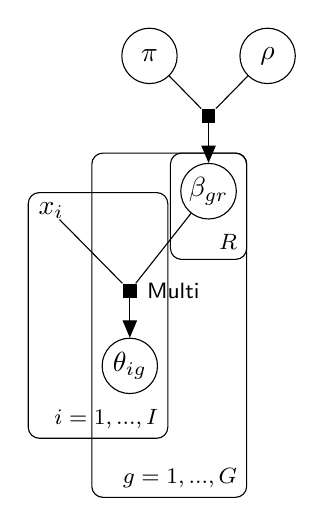
\begin{tikzpicture}%[font=\footnotesize, xscale=1.5]

\node[latent] (theta) {\(\theta_{ig}\)};
\factor[above=0.5 of theta, label=right:Multi]       {theta-f} {} {} {}; %
\node[latent, above=1.5 of theta, xshift=1 cm] (beta) {\(\beta_{gr}\)};
\node[const, above=1.5 of theta, xshift=-1 cm] (x) {\(x_i\)};
\factoredge {x, beta} {theta-f} {theta};

\factor[above=0.5 of beta]       {beta-f} {} {} {}; %
\node[latent, above=1.0 of beta, xshift=-0.75 cm] (pi) {\(\pi\)};
\node[latent, above=1.0 of beta, xshift=0.75 cm] (rho) {\(\rho\)};
\factoredge {pi, rho} {beta-f} {beta};

\plate {i-p} {(x) (theta)} {\(i=1,...,I\)} ;
\coordinate[below=0.75 of theta] (g-p-bottom) ;
\plate {g-p} {(theta) (beta) (g-p-bottom)} {\(g=1,...,G\)} ;

\plate {beta-p} {(beta)} {\(R\)} ;
\end{tikzpicture}
\end{document}
